\documentclass[default]{sn-jnl}% Default

%\raggedbottom

\begin{document}

\title[Effect of pressure on point defects in UMo]{Analyzing the effect of pressure on the properties of point defects in $\gamma$UMo through atomistic simulations}

\author*[1,2]{\fnm{Benjamin} \sur{Beeler}}\email{bwbeeler@ncsu.edu}
\author[3]{\fnm{Yongfeng} \sur{Zhang}}
\author[1]{\fnm{ATM Jahid} \sur{Hasan}}
\author[4]{\fnm{Gyuchul} \sur{Park}}
\author[5]{\fnm{Shenyang} \sur{Hu}}
\author[6]{\fnm{Zhi-Gang} \sur{Mei}}

\affil*[1]{\orgname{North Carolina State University}, \orgaddress{\street{Street}, \city{City}, \postcode{100190}, \state{State}, \country{Country}}}
\affil[2]{\orgname{Idaho National Laboratory}, \orgaddress{\street{Street}, \city{City}, \postcode{10587}, \state{State}, \country{Country}}}
\affil[3]{\orgname{University of Wisconsin, Madison}, \orgaddress{\street{Street}, \city{City}, \postcode{610101}, \state{State}, \country{Country}}}
\affil[4]{\orgname{Purdue University}, \orgaddress{\street{Street}, \city{City}, \postcode{610101}, \state{State}, \country{Country}}}
\affil[5]{\orgname{Pacific Northwest National Laboratory}, \orgaddress{\street{Street}, \city{City}, \postcode{610101}, \state{State}, \country{Country}}}
\affil[6]{\orgname{Argonne National Laboratory}, \orgaddress{\street{Street}, \city{City}, \postcode{610101}, \state{State}, \country{Country}}}

\abstract{
Uranium-molybdenum (U-Mo) alloys in monolithic fuel foil are the primary candidate for the conversion of High-Performance research reactors in the United States. Monolithic fuel is utilized in a plate-type design with a zirconium diffusion barrier and aluminum cladding. These fuel types are unique in that they contain no plenum for the release of fission gases, which, in conjunction with the aluminum cladding, can lead to large stress states within the fuel. The nature of how fundamental processes of radiation damage, including the evolution of point defects, under such stresses occur is unknown. In this work, we present molecular dynamics simulations of the formation energy and diffusion of point defects under applied stress. This work will allow for the implementation of stress-dependent microstructural evolution models of nuclear fuels, including those for both fission gas bubble growth and creep, which are critical to ensure the stable and predictable behavior of research reactor fuels. 
}

\keywords{keyword1, Keyword2, Keyword3, Keyword4}

\maketitle


\section{Introduction}\label{sec1}

A monolithic fuel design with a U-Mo alloy has been selected as the fuel for conversion of the United States High-Performance Research Reactors (HPRRs). This fuel design employs a U-Mo fuel foil, bonded with a zirconium (Zr) interdiffusion barrier, in aluminum (Al) cladding. This design increases the uranium density as compared to the current designs, allowing for a reduced enrichment of the fuel without a reduction in the achievable neutron flux. 

An issue with U-Mo monolithic fuel is the large amount of swelling that takes place during operation \cite{hofman1997}. Such swelling needs to be stable and predictable up to high fission densities. Research reactor fuel types based on U-Mo are unique in their design to stably retain fission gases to high fission densities, and as such there is a relatively high content of fission gas and of fission gas bubbles within the fuel matrix. This large internal pressure of the fuel, combined with the Al cladding constraint and the fixed restraints at either end of the plate, results in a complex stress environment where relatively large compressive stresses are generated and affect the microstructural evolution of the fuel. One notable microstructural effect is the induced creep under irradiation, which has been observed experimentally \cite{kim2013} and explored preliminarily in a computational framework \cite{xmiao2021, xjian2019}. 

A key input into creep models is the behavior of point defects under applied stress. Given an environment where potentially large local stresses are present, if the point defect formation behavior is modified due to a stress field, then the defect evolution, and thus the microstructural evolution, will be affected by that stress field. Mesoscale fuel performance simulations \cite{ye2018, hu2017a} take into account information such as point defect formation energies and diffusion coefficients, but typically assume an Arrhenius relationship that is independent of the stress state. 

\textcolor{red}{
An issue with U-Mo monolithic fuel is the large amount of swelling that takes place during operation \cite{hofman1997}. Such swelling needs to be stable and predictable up to high fission densities. Research reactor fuel types based on U-Mo are unique in their design to stably retain fission gases to high fission densities, and as such there is a relatively high content of fission gas and of fission gas bubbles within the fuel matrix. The importance of swelling in addition to the unique fuel environment has led to a variety of experimental studies characterizing the swelling behavior in U-Mo fuels \cite{rest2009, kim_anl08, meyer2002, kim2013}, which has led to the development of a swelling correlation as a function of fission density from Argonne National Laboratory (ANL) \cite{kim2011} and Idaho National Laboratory (INL) \cite{umo_prelim_report2017}. A 2015 post-irradiation examination (PIE) report \cite{afip6report} from Williams, et al. showed higher swelling in U-10Mo (alloy composition is provided in weight percent unless otherwise noted) fuels at fission densities much lower than previously observed. This accelerated fuel swelling behavior could lead to early fuel failure and was not captured by the ANL correlation. As such, a more mechanistic fuel swelling model is needed in order to predict swelling behavior of U-Mo fuels under both typical operating conditions, as well as transients, accident scenarios and different reactor environments.
Recently, substantial effort has been made on mesoscale models to describe the swelling behavior of U-Mo fuels \cite{liang2018, liang2018a, liang2017, liang2016, ye2018, hu2017a, hu2016, hu2016a}. These models rely on phase-field and/or rate theory descriptions of material systems in order to model swelling on realistic timescales on a microstructural level. These simulation methodologies include a number of parameters that are either fit to limited experimental data, calculated from lower length scale modeling methodologies, or assumed based on other material systems. One such assumption is the diffusion of species at low temperature. Research reactor fuels operate at relatively low temperatures, within a range of 150\textdegree C to 350\textdegree C. Intrinsic, thermal diffusion is relatively limited at these temperatures and no such experimental data on diffusive behavior in this temperature range exists. 
A number of high temperature experimental studies have been conducted on interdiffusion, tracer diffusion and self-diffusion in the U-Mo system. Adda, et al. determined the interdiffusion coefficient of U-Mo from 1123 K to 1323 K and subsequently determined the self-diffusion coefficient of uranium with 10 atomic percent Mo \cite{adda1962}. Lundberg determined interdiffusion coefficients from 1400 K to 1525 K for a range of high Mo content systems (higher than U-10Mo) \cite{lundberg1989}. Huang, et al. calculated interdiffusion and intrinsic diffusion of U-Mo alloys from 923 K to 1273 K via diffusion couples \cite{huang2013}. All of these experimental studies agree that in U-rich U-Mo alloys, U diffuses more rapidly than Mo and that the interdiffusion coefficient is reduced with the addition of Mo. However, none of these studies investigated low temperature systems due to the difficulties in obtaining data due to reduced intrinsic diffusion of species at low temperatures. Thus, the diffusion data are often extrapolated from high temperature systems to low temperature as a means of estimation. Additionally, there are no experimental studies of fission gas diffusion in U-Mo alloys. 
For the study of self- and fission gas diffusion in UO$_2$, the nuclear fuel type typically utilized in commercial reactors in the U.S., the total diffusion coefficient is typically broken down into three component parts: 1) intrinsic diffusion (D$_1$), 2) radiation enhanced diffusion (D$_2$), and 3) radiation driven diffusion (D$_3$). Each of these constituent parts is dominant in a given temperature regime, as was initially discussed by Turnbull \cite{turnbull1982} and computationally investigated by Andersson, et al. \cite{andersson2014} and Cooper, et al. \cite{cooper2016}, and others \cite{matthews_cluster_2019, perriot_atomistic_2019, wormald2015, martin2009}. Given the low operating temperatures of research reactors, it is expected that radiation driven diffusion will be a critical component of the total diffusion. No experimental or computational studies have been performed to investigate radiation driven diffusion in U-Mo or U-Mo-Xe systems.
In this work, molecular dynamics simulations are performed to determine the radiation driven diffusion of U, Mo and Xe in U-Mo nuclear fuels. Diffusion coefficients for each species are determined over a range of temperatures and compositions. Updated diffusion coefficients are presented that are applicable under irradiation that incorporate both intrinsic and radiation driven diffusion. 
}
\section{Computational Details}\label{sec2}

Molecular dynamics simulations are performed utilizing the LAMMPS \cite{plimpton1995} software package and the U-Mo angular dependent potential (ADP) \cite{smirnovaADP}. A 14x14x14 supercell consisting of 5488 atoms is constructed in a body-centered cubic (bcc) structure, which is the relevant crystal structure for UMo research reactor fuels. Relaxation is performed in an NPT-ensemble, relaxing each x, y, and z component individually, with a damping parameter of 0.1 ps. A Nose-Hoover thermostat is utilized with the damping parameter set to 0.1 ps. Systems are investigated over a range of temperatures, from 600 K up to 1200 K, in increments of 200 K. This temperature range was chosen due to the inherent properties of the potential, in that below 600 K $\gamma$U becomes mechanically unstable and above 1200 K the crystal structure is approaching the melting point. Systems are relaxed for 100 ps, with volumes averaged over the final 50 ps. The equilibration is performed at a given pressure, ranging from -10 kbar to +10 kbar (-1 GPa to +1 GPa) in increments of 5 kbar. This pressure range should exceed any expected stress state of the fuel, and as such should present the possibilities of extreme behavior on defect evolution. Additionally, trends in behavior can be determined and explored at the pressures of interest. The sign of the pressure indicates compressive or tensile stress, in that a negative pressure is that which is applied to the supercell, resulting in a tensile stress, while a positive pressure results in a compressive stress. Eight individual compositions are investigated, including pure U and pure Mo, U-5Mo, U-10Mo, U-15Mo, U-30Mo, U-50Mo, and U-70Mo. All compositions are given in weight percent unless otherwise noted. This variation in composition allows for analysis for a wide range of U-Mo systems, including all relevant compositions in monolithic fuel.  

Following the relaxation, the system is scaled to the time-averaged volume as determined from the NPT simulation. A further relaxation of 50 ps is performed, the final 25 ps of which is utilized to determine average energies. A defect (vacancy or interstitial) is then inserted into the system and allowed to evolve for 50 ps, the final 25 ps of which is utilized to determine average energies. For an alloy composition, a proportional number of atoms are either removed or inserted, depending on the defect type, to closely maintain the stoichiometry of the system. For interstitials, an atom is randomly deposited into the supercell, provided that no other atom is within 1.5 \AA, allowing for a random sampling of the entire supercell and all possible local configurational environments. To ensure statistical certainty of the results, 2000 simulations for each defect type, pressure, and temperature are performed, similar to the approach in Ref. \cite{zhang2021}. This generates a standard error of the mean for defect formation energy calculations of approximately 0.05 eV. 

The formation energy is defined as:
\begin{equation}
 E_f= E_f^{def} -  \frac{(n\pm1)}{n}E_f^{bulk}
\end{equation}
\noindent where n is the total number of atoms in the system with no defects and E$_f^{bulk}$ or E$_f^{def}$ is defined as:
\begin{equation}
E_f^{def/bulk}= E^*- N_U \times E_U - N_{Mo} \times E_{Mo} 
\end{equation}
\noindent where E$^*$ is the total energy of the system either with or without a defect, N$_U$ is the number of uranium atoms in the system, E$_U$ is the energy per atom of U, N$_{Mo}$ is the number of molybdenum atoms in the system, and E$_{Mo}$ is the energy per atom of Mo. This formalism critically takes into account the non-zero formation energy of the alloy compound. The energy is defined for a given temperature and pressure, according to the system of interest. 

The diffusion coefficient as a function of temperature and pressure is determined for the same sets of pressures as described above, but only for temperatures at 800 K and above. This is due to the limited thermal diffusion at low temperatures on a molecular dynamics time scale. The number of compositions is reduced to five (bcc U, U-5Mo, U-10Mo, U-15Mo, and bcc Mo) due to the computational cost associated with diffusion calculations. However, the primary concentration range of interest for U-Mo monolithic fuel is encompassed by this compositional range. An identical procedure is followed for the implementation of defects for investigation of diffusion as that which was followed for the investigation of defect energies. Following the defect insertion and relaxation, an additional evolution step of 10 ns was performed, over which the mean-squared displacement (msd) of the total system, and of each elemental species, was tracked. Over this 10 ns trajectory, three overlapping trajectories were obtained, each of length 6 ns, in order to subsample the trajectory and increase the statistics of the dataset. Additionally, five unique simulations are performed for each temperature, composition, and pressure, to further ensure statistical significance of the results. The diffusion coefficient is determined from the slope of the msd as a function of time via Einstein's equation:
\begin{equation}
D = \frac{r^2}{2dt} 
\end{equation}
\noindent where $r^2$ is the msd, $d$ is the dimensionality (in this case three), and $t$ is the time. 

\section{Results}\label{sec3}
\subsection{Point Defect Formation Energies}
The temperature dependence of the nominal pressure defect formation energies is shown in Figure \ref{fig:A} A and B. For interstitials, the temperature dependence undergoes an inflection point as a function of composition, in that in the U-rich regime, higher temperatures lead to higher interstitial energies, while in the Mo-rich regime higher temperatures lead to lower interstitial energies. This transition occurs at approximately 30 atomic percent or 15 weight percent Mo. For vacancies, the trend of defect energy with temperature is consistent across the compositional spectrum, in that higher temperatures lead to higher defect energies. The sensitivity of this temperature dependence varies with composition, with the most temperature-sensitive compositions in the U-rich regime. The absolute magnitude of the defect formation energies should also be noted, in that for U-rich alloys, interstitial formation energies are lower than vacancy formation energies, in accordance with previous work \cite{beeler2010,beelerAIMD,smirnova2015} and the concept of self-diffusion via an interstitialcy mechanism \cite{park2021}. This trend is reversed to its typical order at high Mo concentrations, where the vacancy formation energy is lower than the interstitial formation energy. This is the first time that the entire compositional range has been explored and this inflection has been identified. The inflection occurs at approximately 50\% Mo content, but varies based upon temperature, where at higher temperatures the vacancy formation energy does not become less than the interstitial formation energy until above 70\% Mo. 


An example of the formation energy as a function of pressure for U-10Mo at 1200 K is shown in Figure 108. In correspondence with prior work [118] on defect energetics in U-Mo systems, the interstitial formation energy for the nominal case is less than 1 eV (0.62 eV) and the vacancy formation energy is significantly high than the interstitial formation energy (1.92 eV). Considering slight differences in methodology, this is reasonable agreement with the previous literature. From Figure 108, it can be seen that as vacancies and interstitials exhibit opposite trends as a function of applied pressure, as would be expected. As a crystal structure is compressed (positive pressure), atoms are closer together than in the equilibrium case. As such, it would be expected that a vacancy is more easily formed in the compressive state, and this is indeed observed. In the tensile state (negative pressure), atoms are farther apart than at equilibrium and there is additional space between the atoms. In this case, it would be expected that it is comparatively easier for an interstitial for form, and this is indeed observed. There is a generally linear dependence of the formation energy on the applied pressure in the system, with vacancies exhibiting a negative slope and interstitials exhibiting a positive slope. The total magnitude change in the defect formation energy for this case is 0.14 eV and 0.17 eV for interstitials and vacancies, respectively. This corresponds to approximately a 4-5X higher defect concentration across this pressure range. 

Generalizing to the U-Mo system, the interstitial and vacancy formation energies as a function of composition and pressure at 1200 K are shown in Figure 109 and Figure 110, respectively. The defect formation energies vary in a similar manner as a function of composition, with a minimum in the formation energy at 20-30 atomic percent. Interestingly, this is the target composition (22 atomic percent) for U-Mo monolithic fuel. Additionally, defect energies are at a maximum for the pure bcc Mo system for both interstitials and vacancies. The pressure sensitivity is not uniform for defect type and composition, in that interstitials are the most sensitive to pressure at intermediate compositions (40-60 atomic percent), while vacancies are the most sensitive to pressure in the U-rich regime. The trends of applied pressure observed in Figure 108 hold for all compositions. 

The application of pressure does affect the temperature dependence of defect formation energies, nor does the temperature affect the trends of applied pressure on defect formation energies. However, it does appear that at lower temperatures, the effects of pressure on interstitial formation energy are slightly dampened. Averaging over the entire compositional regime, an applied pressure of 10(-10) kbar at 1200 K produces a 11(9)\% increase(decrease) in the formation energy. At 600 K, an applied pressure of 10(-10) kbar produces a 6(7)\% increase(decrease) in the formation energy. 

It is found that generally, vacancies are much less sensitive to pressure than interstitials, and that sensitively is not significantly affected by the temperature of interest. On average, an applied pressure of 10(-10) kbar produces a 3\% increase(decrease) in the vacancy formation energy. Since the magnitude of the vacancy formation energy is larger than the magnitude of the interstitial formation energy, the absolute (not relative) change in the defect formation energy with applied pressure is approximately the same for both interstitials and vacancies. Under reasonable applied bulk pressures below the yield point ($<$100 MPa), negligible deviations in the defect formations are observed. However, in circumstances where the pressures may be quite large, e.g., in the area surrounding a highly pressurized nanometer-sized bubble, statistically significant changes in the local defect formation energy could be observed, potentially altering fission gas bubble evolution and creep behaviors.

\begin{figure}[htbp]
\begin{center}
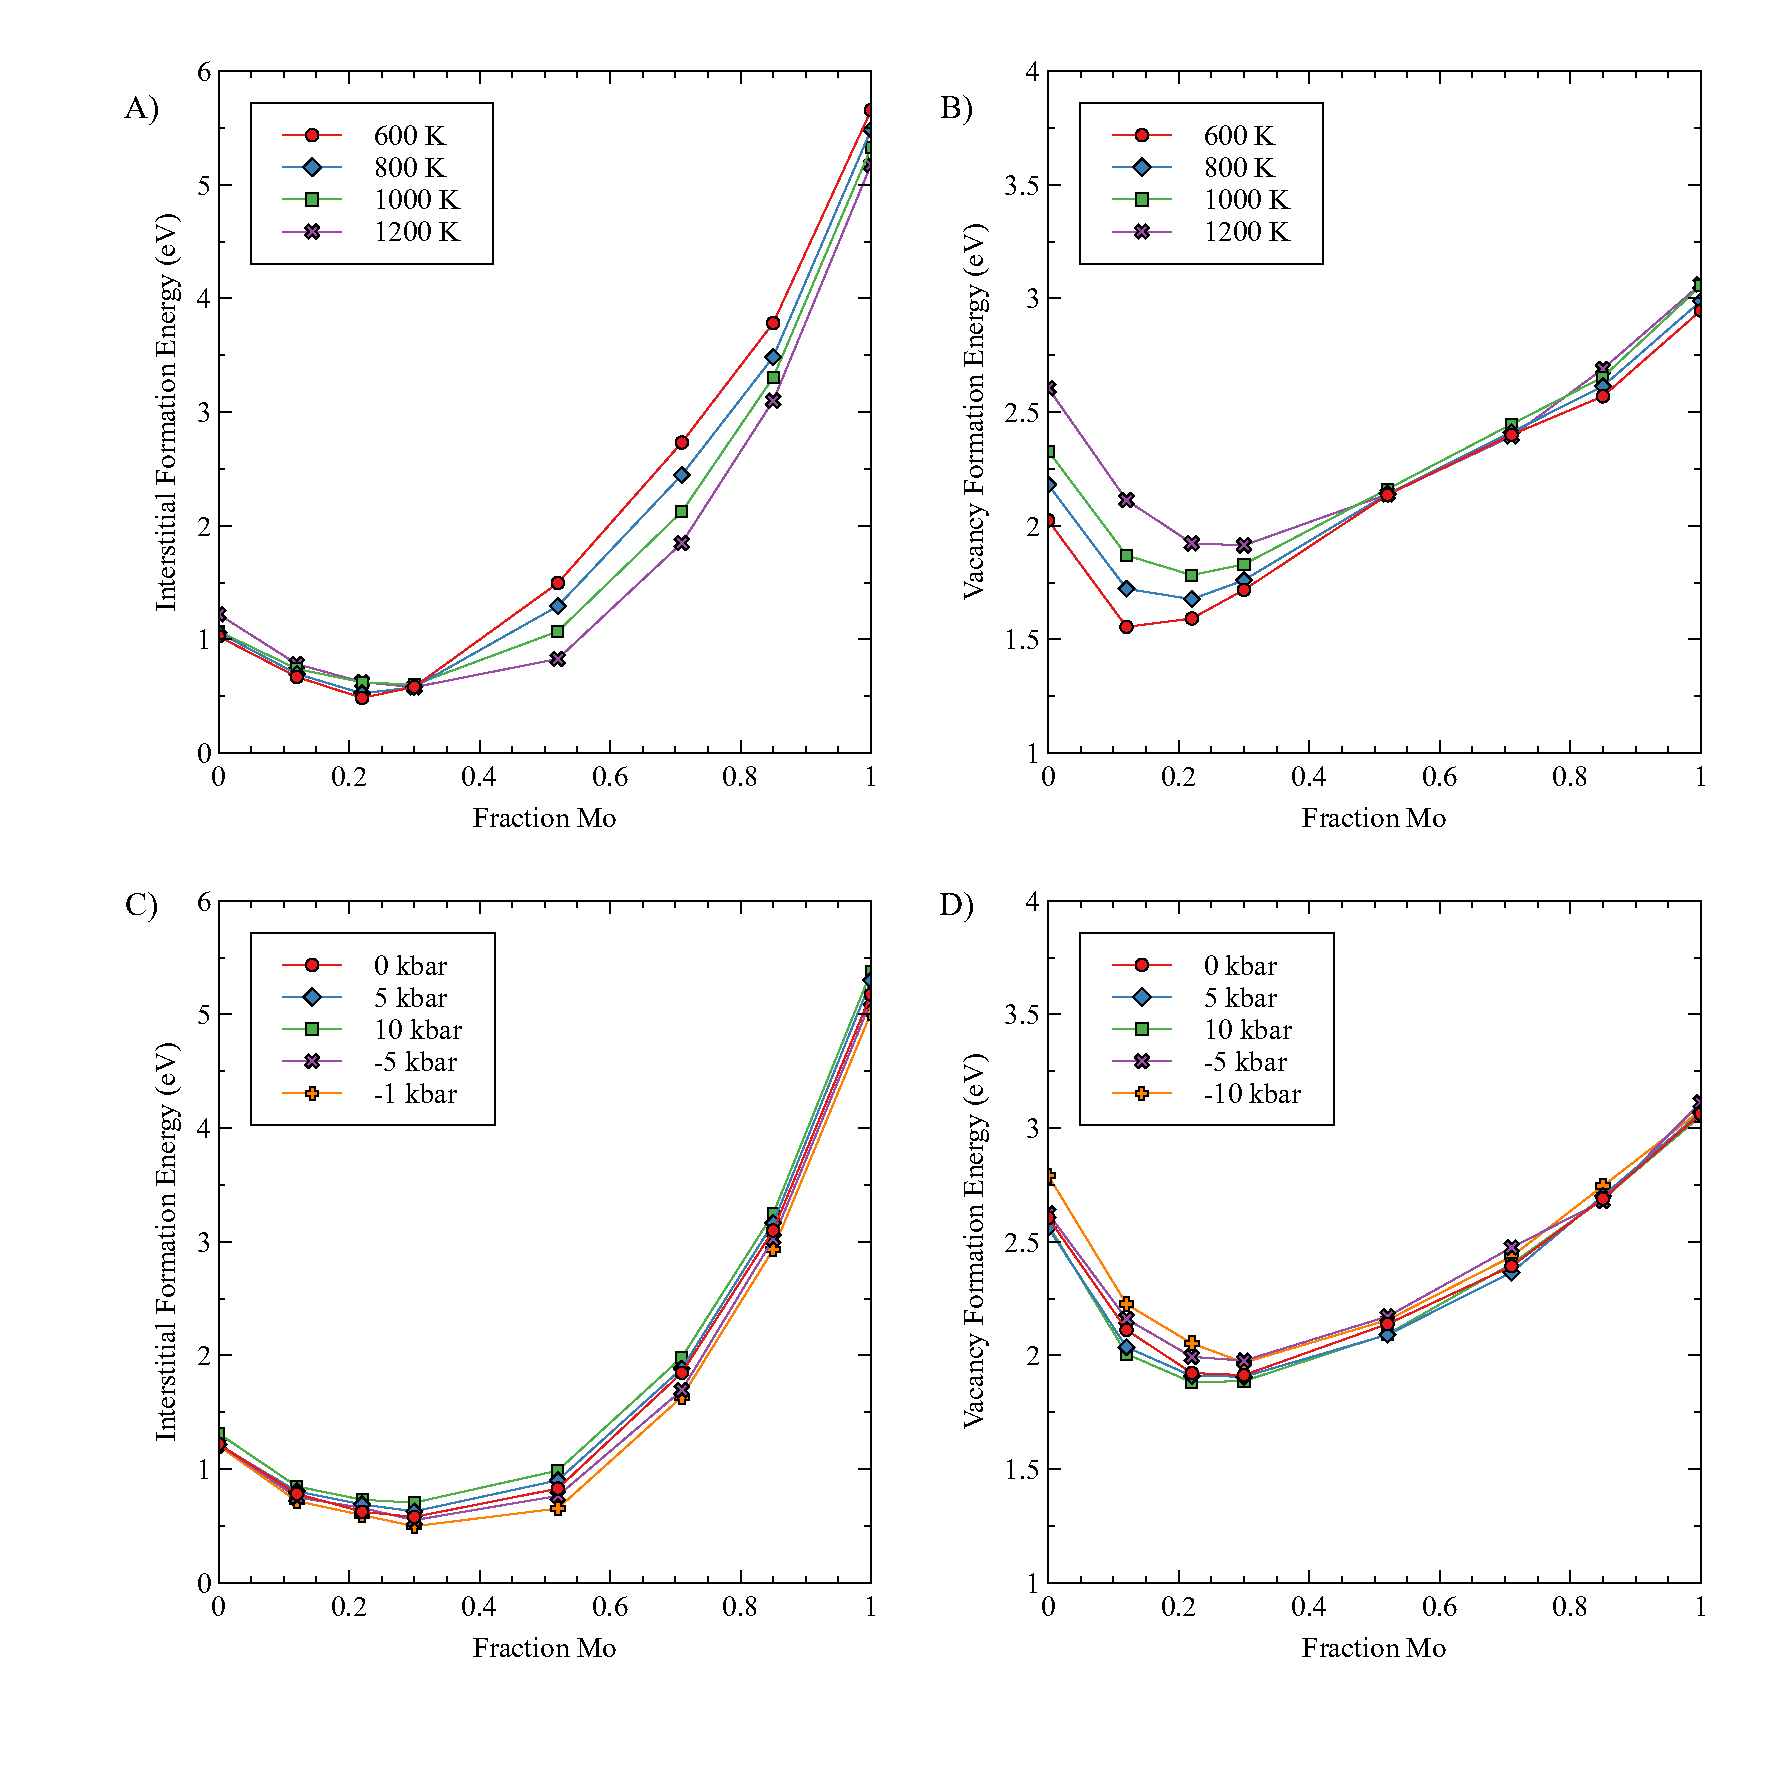
\includegraphics[width=0.9\textwidth]{figA.pdf} 
\caption{this is the caption}
\label{fig:A}
\end{center}
\end{figure}

\subsection{Point Defect Diffusion}
The diffusion coefficient of interstitials and vacancies as a function of composition and temperature is shown in Figure 112. As previously observed [118], the defect diffusion coefficient varies as a function of composition, generally decreasing with an increasing content of Mo. However, there is an inflection point above U-15Mo for interstitials, as the interstitial diffusion coefficient for bcc Mo is higher than that of U-15Mo. For vacancies, there is no evident turnaround point. This is consistent with existing literature. 

The diffusion coefficient for vacancies and interstitials as a function of pressure in U-10Mo at three temperatures is shown in Figure 113. There is minimal variation as a function of applied pressure, but clear trends do present themselves. As the pressure increases and the system is in compression, the diffusion coefficient tends to decrease for both vacancies and interstitials. Thus, there is a clear distinction between pressure effects on the formation energy and pressure effects on the diffusion. The diffusion will consist of a series of components, including the migration barrier and the jump frequency.  The migration barrier can be elucidated from the slope of the Arrhenius fit to the diffusion data. Such plots are shown in Figure 114 for U-10 Mo for all five pressures of interest. 

There is very minimal variation in the migration energy as a function of pressure. The difference between the maximum and minimum predicted migration barriers is 0.02 eV, which is less than the presumed statistical certainty. As such, it can be supposed that applied pressure produces no statistically significant change in the migration barrier. To cause a slight reduction in the diffusion coefficient, it is then assumed that a compressive state reduces the attempt frequency of both types of defects, thereby reducing the magnitude of the defect diffusion. However, such changes in the diffusion coefficient are on the order of less than 10\% for 500 MPa (5 kbar). Additionally, it appears that the magnitude of the pressure dependence on interstitial diffusion decreases as the temperature decreases, taken from the slope in Figure 113. Given that research reactor temperatures are below the investigated temperature range, that expected pressures are significantly below the investigated range, and extrapolating the observed trends to lower temperatures, it is presumed that effectively negligible effects on point defect diffusion from the system pressure will be observed and can thus be safely ignored. 

\section{Discussion}\label{sec4}
This work investigated how the application of hydrostatic tension and compression affects the formation energy and diffusion coefficient of interstitials and vacancies in U-Mo as a function of pressure, temperature, and composition. On average, the maximum applied pressure of 10 kbar produces a 6\% increase in the interstitial formation energy and a 3\% decrease in the vacancy formation energy. Under reasonable applied bulk pressures below the yield point (<100 MPa), negligible deviations in the defect formations are observed. Also, applied pressures should yield negligible variation on point defect diffusion at relevant temperatures and pressures. There are impacts of the applied pressure on defect formation and diffusion and clear trends can be observed, but these effects are sufficiently small, even at large pressures, that they likely can be neglected for practical purposes. However, in circumstances where the pressures may be quite large, e.g., in the area surrounding a highly pressurized nanometer-sized bubble, statistically significant changes in the local defect formation energy and diffusion coefficient could be observed, potentially altering fission gas bubble evolution and creep behaviors.

\section{Acknowledgements}\label{sec5}
This work was supported by the U.S. Department of Energy, Office of Material Management and Minimization, National Nuclear Security Administration, under DOE-NE Idaho Operations Office Contract DE-AC07-05ID14517. This manuscript has been authored by Battelle Energy Alliance, LLC with the U.S. Department of Energy. The publisher, by accepting the article for publication, acknowledges that the U.S. Government retains a nonexclusive, paid-up, irrevocable, worldwide license to publish or reproduce the published form of this manuscript, or allow others to do so, for U.S. Government purposes. This research made use of the resources of the High Performance Computing Center at Idaho National Laboratory, which is supported by the Office of Nuclear Energy of the U.S. Department of Energy and the Nuclear Science User Facilities.

\section{Conflict of Interest}\label{sec6}
The authors declare no competing financial interest.


\bibliographystyle{abbrv}
\bibliography{beelerbib}

\end{document}
